% !TeX spellcheck = en_GB
\chapter{Subfactors and fusion categories}
\label{ch:subfactor}

The study of subfactors \cite{araki_subfactors_1994,Jones1997} has always been connected to physics, more precisely, quantum field theory. Mathematical investigations of these fields have led to a conjectured correspondence between subfactors and Conformal Field Theories (CFTs) by Jones \cite{Jones1990,Jones2014}, which builds on original work of Doplicher and Roberts \cite{Doplicher1989} and was later substantiated by Bischoff \cite{Bischoff2015,Bischoff2016}. Evidence for this conjecture was found, for example, in \cite{Calegari2010,Xu2017}. However, a proof of this conjecture is far from being in sight, since there are still numerous gaps. One example of a subfactor with no known counterpart CFT is the Haagerup subfactor \cite{Haagerup1994}, the smallest (finite-depth, irreducible, hyperfinite) subfactor with index above four. Although some evidence for the existence of such a CFT was provided by Evans and Gannon \cite{Evans2011}, the proof of the existence of the CFT is still an open problem.

The Haagerup subfactor provides the motivating example for most of the work that is done in this thesis. Every finite-depth, irreducible, hyperfinite subfactor gives rise to two fusion categories (its \emph{principle even} and \emph{dual even} parts). In case of the Haagerup subfactor, there is a third category that is Morita equivalent, but not equivalent to these two categories. This category, which is discussed in detail in the next chapter, will be the basis of most of the lattice constructions that are done in the second part of this thesis. 

In this chapter we explain how fusion categories can be constructed from a subfactor. We begin with giving the most important definitions to understand subfactors in terms of operator algebras and their classification via the index before we explore the connection to fusion categories. We also explain the connection between the different fusion categories in terms of algebra objects and module categories and show how to find all subfactors related to a given fusion category. We end this chapter by presenting the construction of the \emph{centre} of a fusion category which provides a way to get a modular tensor category from a fusion category.


\section{Fusion categories from subfactors}

In this section, we explain the connection between subfactors and fusion categories. Since we only use the language of fusion categories in the constructions explained later in this thesis, we only briefly talk about subfactors and mostly focus on the corresponding fusion categories. For a detailed introduction to the theory of subfactors, see for example \cite{Jones1997}. In the following, we use some notions and theorems from basic abstract algebra and operator algebra, such as the standard algebraic tensor product or modules over algebras, which are not introduced here in detail since they can be found in any standard textbook on the subject, for example in \cite{Jacobson2009a,Jacobson2009b}. For a more detailed treatment of von Neumann algebras, see the notes by Vaughan Jones \cite{JonesvNA}. In this thesis, we focus on the definitions and explanations of the corresponding categorical notions of these objects.

\begin{defn}[von Neumann algebra]
	A von Neumann algebra\index{von Neumann algebra} is a self-adjoint subalgebra $M$ of $\mathcal{L}(\Hi)$ (the algebra of all bounded operators on a Hilbert space $\Hi$) that satisfies $M=(M')'$, where
		\begin{equation}
			M'=\{x'\in\mathcal{L}(\Hi):x'x=xx'\text{ for all }x\in M\}
		\end{equation}
	is the commutant of $M$.
\end{defn}

\begin{defn}[Factor]
	A von Neumann algebra $M$ with trivial centre (i.e., it only contains multiples of the identity operator) is called a factor\index{factor}. 
%	A subfactor\index{subfactor} $S$ is an inclusion $S\subseteq R$.
\end{defn}

\begin{defn}[Subfactor]
	A subfactor\index{subfactor} of a factor $M$ is a subalgebra $N\subseteq M$ such that $N$ is also a factor and $N$ contains the identity element of $M$. The subfactor $N$ is said to be irreducible\index{irreducible subfactor} if it has \emph{trivial relative commutant}, i.e., if $N'\cap M=\mathbb{C}$.
\end{defn}

To classify factors, the notion of minimal and finite \emph{projections} in a von Neumann algebra is important.

\begin{defn}[Projection]
	\index{projection}
	An operator $p$ in a von Neumann algebra $M$ is called a projection if $p=pp=p^*$. $p$ is called \emph{minimal} if there is no other projection $q$ with $0<q<p$. It is called \emph{finite} if there is no projection $q<p$ that is equivalent to $p$.
\end{defn}

\begin{defn}
	A factor $M$ is said to be finite\index{finite factor} if the multiplicative identity of $M$ (which always exists) is a finite projection in $M$.
\end{defn}

With these definitions at hand, we can introduce the classification of factors in the way it was done by Murray and von Neumann \cite{Murray1936}: A factor $M$\index{classification of factors} is said to be of
	\begin{enumerate}
		\item type $I$ if there exists a non-zero minimal projection in $M$.
		\item type $II$ if it contains non-zero finite projections and is not of type $I$. If the multiplicative identity of $M$ is a finite projection, then $M$ is of type $II_1$, otherwise it is of type $II_\infty$.
		\item type $III$ if no non-zero projection of $M$ is finite.
	\end{enumerate}
It can be shown (see, for example, \cite{Takesaki1979}) that every factor is either of type $I$, type $II_1$, type $II_\infty$, or type $III$.

We are especially interested in type $II_1$ factors since they have the convenient property that they are equipped with a unique trace and, as we will see, they give rise to fusion categories. To classify subfactors of type $II_1$ factors one can define an \emph{index}, and the trace is the key to this definition because it allows us to associate a dimension to vector spaces on which the factor acts. Let $M$ be a type $II_1$ factor with trace $\Tr_M:M\to\mathbb{C}$. For $x,y\in M$, the trace defines an inner product on $M$ via
	\begin{equation}
		\langle x,y\rangle=\Tr_M(y^* x).
	\end{equation}
The completion of $M$ with respect to the inner product defined above then yields a Hilbert space and is denoted $L^2(M)\equiv L^2(M,\Tr_M)$. The Hilbert space $L^2(M)$ is automatically a left-module over $M$ and a right module over $M^\mathrm{op}$ (which is the von Neumann algebra which is defined to be $M$ as complex vector space, but with the opposite multiplication), hence it is an $M$-bimodule (see \cite{Thom2006}). We call a Hilbert space which is at the same time a bimodule over $M$ a \emph{Hilbert bimodule}\index{Hilbert bimodule} (left and right Hilbert modules are defined analogously). The index of a subfactor is then defined as follows:
	\begin{defn}
		For a type $II_1$ factor $M$ and a subfactor $N\subseteq M$ the index\index{index}, denoted $[M:N]$, measures the dimension of $M$ as an $N$-module:
			\begin{equation}
				[M:N]=\dim_N L^2(M).
			\end{equation}
	\end{defn}
The precise definition of the dimension $\dim_N L^2(M)$ requires more mathematical details than are necessary for the purpose of this thesis, therefore we do not state it here but refer to \cite{Jones1997}, or, for a detailed mathematical treatment, \cite{Lueck2002}. Note that the index is equal to one if and only if $N=M$. 

Before we go into more detail about the possible values the index can take and the classification of subfactors that comes with it, we introduce an important example of a type $II_1$ factor: the \emph{hyperfinite} type $II_1$ factor\index{hyperfinite type 21 factor@hyperfinite type $II_1$ factor}, denoted $\mathcal{R}$. This factor is the unique smallest infinite-dimensional factor in the sense that it can be embedded in every other infinite-dimensional factor, and any infinite-dimensional factor contained in $\mathcal{R}$ is isomorphic to $\mathcal{R}$ (see \cite{Connes1976}). We can think of this factor as the inductive limit of inclusions of $n\times n$-matrices $\overline{\lim_{n\to\infty}M_{2^n\times2^n}(\mathbb{C})}$, i.e., the sequence
	\begin{equation}
		M_{2\times 2}\subseteq M_{4\times 4}\subseteq M_{8\times 8}\subseteq\dots\subseteq M_{2^n\times 2^n}\subseteq M_{2^{n+1}\times 2^{n+1}}\subseteq\dots
	\end{equation}
This means that we embed the $2\times 2$ matrices into $4\times 4$ matrices by building a block diagonal $4\times 4$ matrix, then embed the $4\times 4$ matrices by building a block diagonal $8\times 8$ matrix and so on. 
%The hyperfinite type $II_1$ factor $\mathcal{R}$ has two types of subfactors: The subfactor is either $\mathbb{C}$ or it is isomorphic to $\mathcal{R}$ itself. 

We now come back to the index of a subfactor. An important result by Jones \cite{Jones1983} gives the possible values the index can take:
	\begin{thm}
		Let $N\subseteq M$ be an inclusion of type $II_1$ factors. Then	
		\begin{equation}
			[M:N]\in\left\{4\cos^2\frac{\pi}{n}|n=3,4,\dots\right\}\cup[4,\infty],
		\end{equation}
		which means that the indices less than four accumulate at four and have gaps in between. Conversely, for any $\lambda\in\{4\cos^2\frac{\pi}{n}|n=3,4,\dots\}\cup[4,\infty]$ there exists a type $II_1$ factor $M$ and a subfactor $N$ with $[M:N]=\lambda$.
	\end{thm}
Furthermore, it can be shown that every index shows up as a possible index in the case where $M\cong N\cong\mathcal{R}$ is the hyperfinite type $II_1$ factor. The index can be visualized as follows:
	\begin{figure}[H]
		\centering
		\begin{tikzpicture}
			\draw[->,>=stealth] (0,0) -- (10,0); 
			\draw (0,-0.25) -- (0,0.25);
			\draw (1,-0.25) -- (1,0.25);
			\draw (2,-0.25) -- (2,0.25);
			\draw (3,-0.25) -- (3,0.25);
			\draw (4,-0.25) -- (4,0.25);
			\node at (0,-0.5) {$0$};
			\node at (1,-0.5) {$1$};
			\node at (2,-0.5) {$2$};
			\node at (3,-0.5) {$3$};
			\node at (4,-0.5) {$4$};
			\foreach \a in {0,0.25,0.5,...,4}{
				\draw (\a,0) -- (\a,-0.125);			
			}
			\foreach \a in {1., 2., 2.61803, 3., 3.24698, 3.41421, 3.53209, 3.61803, 3.68251, 3.73205, 3.77091, 3.80194, 3.82709, 3.84776, 3.86494, 3.87939, 3.89163, 3.90211, 3.91115, 3.91899, 3.92583, 3.93185, 3.93717, 3.94188, 3.94609, 3.94986, 3.95324, 3.9563}{
				\node at (\a,0) {\color{LinkColor} $\bullet$};
			}
			\draw[very thick, color=LinkColor] (4.125,-0.25) -- (4,-0.25) -- (4,0.25) -- (4.125,0.25);
			\draw[thick, color=LinkColor] (4,0) -- (9.915,0);
		\end{tikzpicture}
	\end{figure}

For subfactors with index smaller than four, there is a complete classification via the so-called \emph{standard invariant} \cite{Popa1990,Popa1994}. For subfactors with index four and above, i.e., all those who have an index in the continuous part, there is no complete classification yet. The main complication that arises here is that there are many subfactors which satisfy some technical condition called \emph{non-amenability}, where the results that Popa found cannot be applied. In \cite{Jones2013}, amenable subfactors with index between four and five are classified, but the authors point out that a classification beyond index five is still an open question and it is not even clear whether the question itself makes sense beyond this point. The subfactor that gives rise to the fusion categories we study in this thesis is the one with the smallest index between four and five, namely $\frac{5+\sqrt{13}}{2}$, and it is called the \emph{Haagerup subfactor}. But before we present it in more detail, we discuss how fusion categories can arise from subfactors.

\subsection*{The principal graphs.}

An algebra is a bimodule over any of its subalgebras, and bimodules over an algebra have tensor product structure given by the Connes fusion product\index{Connes fusion product} (see \cite{Connes80,Thom2006}). This is constructed as follows: Consider a left $A$-module $K$. We define the space
	\begin{equation}
		\mathcal{D}(K,\Tr_A)=\Hom_{-A}\left(L^2(A,\Tr_A),K\right)
	\end{equation}
of linear operators from $L^2(A,\Tr_A)$ to $K$ that are compatible with the left $A$-action (i.e., which are left $A$-module homomorphisms). The space of operators $\mathcal{D}(K,\Tr_A)$ is naturally a bimodule over $A$ itself (like every space of module homomorphisms), hence we can define the \emph{Connes fusion} of two $A$-modules $K$ and $L$ via the tensor product of corresponding operator spaces:
	\begin{equation}
		\mathcal{D}(K,\Tr_A)\otimes_A \mathcal{D}(L,\Tr_A).
	\end{equation}
Similar to the construction of $L^2(A,\Tr_A)$, we need to define an inner product on this space and take the completion with respect to this inner product in order to get a Hilbert bimodule (and not just a bimodule). For the construction of this inner product, we first define an $A$-valued inner product on $\mathcal{D}(K,\Tr_A)$ in the following way: For two operators $x,y\in\mathcal{D}(K,\Tr_A)$, we define
	\begin{equation}
		(x,y)=y^* x,
	\end{equation}
which is an element in $A$. The inner product on $\mathcal{D}(K,\Tr_A)\otimes_A \mathcal{D}(L,\Tr_A)$ is then defined as
	\begin{equation}
	\label{eq:inner}
		\langle x_1\otimes y_1,x_2\otimes y_2\rangle=\Tr_A\left((x_1,x_2)\triangleright y_1,y_2\right),
	\end{equation}
where $(x_1,x_2)\triangleright y_1$ denotes the left action of the operator $(x_1,x_2)\in A$ on $y_1$ regarded as an $A$-bimodule element. Finally, the Connes fusion 
	\begin{equation}
		K\otimes'_A L
	\end{equation}
of two Hilbert bimodules $K,L$ is defined as first forming the space $\mathcal{D}(K,\Tr_A)\otimes_A \mathcal{D}(L,\Tr_A)$ and then taking the completion with respect to the inner product defined in \cref{eq:inner}.

We can now apply the Connes fusion product to subfactors. For a subfactor $N\subseteq M$, it is natural to consider the tensor product 
	\begin{equation}
		M_k=M\otimes_N M\otimes_N M\dots\otimes_N M
	\end{equation}
with $k$ copies of $M$ in the tensor product. It is now possible to decompose $M_k$ into $N-N$, $M-M$, $N-M$, and $M-N$ bimodules, which allows us to extract finite-dimensional data from the, in general, infinite-dimensional $M_k$. Following the notions of \cite{Ocneanu1989} and \cite{Haagerup1994}, we define the four types of bimodules as follows: The $N-M$ bimodule is denoted
	\begin{equation}
		\alpha={}_NL^2(M)_M,
	\end{equation}
given by 
	\begin{equation}
		\alpha(n,m)x=nxm, \hspace{10pt}n\in N,\ m\in M,\ x\in L^2(M).
	\end{equation}
Similarly, the $M-N$ bimodule $\bar{\alpha}={}_ML^2(M)_N$ is given by
	\begin{equation}
		\bar{\alpha}(m,n)x=mxn, \hspace{10pt}m\in M,\ n\in N,\ x\in L^2(M).
	\end{equation}
Moreover, we denote $\epsilon_N={}_NL^2(M)_N$ and $\epsilon_M={}_ML^2(M)_M$ the trivial $N-N$ and $M-M$ bimodule, respectively. To simplify the notation, we omit the tensor product between bimodules: For two bimodules $\beta$ and $\gamma$ given by
	\begin{equation}
		\beta={}_P H_Q,\hspace{10pt} \gamma={}_Q K_R,\hspace{10pt} P,Q,R\in\{M,N\}
	\end{equation}
let $\beta\gamma$ denote the $P-R$ bimodule $\beta\otimes_Q\gamma$. With this notation at hand, we can now define the following four sets:
	\begin{enumerate}
		\item Principal even part\index{principal even part} $\Gamma_\mathrm{even}=$ the set of irreducible $N-N$ bimodules occurring in the decompositions of $\epsilon_N,\alpha\bar{\alpha},(\alpha\bar{\alpha})^2\dots$
		\item Principal odd part\index{principal odd part} $\Gamma_\mathrm{odd}=$ the set of irreducible $N-M$ bimodules occurring in the decompositions of $\alpha,\alpha\bar{\alpha}\alpha,\alpha(\bar{\alpha}\alpha)^2\dots$
		\item Dual even part\index{dual even part} $\Gamma'_\mathrm{even}=$ the set of irreducible $M-M$ bimodules occurring in the decompositions of $\epsilon_M,\bar{\alpha}\alpha,(\bar{\alpha}\alpha)^2\dots$
		\item Dual odd part\index{dual odd part} $\Gamma'_\mathrm{odd}=$ the set of irreducible $M-N$ bimodules occurring in the decompositions of $\bar{\alpha},\bar{\alpha}\alpha\bar{\alpha},\bar{\alpha}(\alpha\bar{\alpha})^2\dots$
	\end{enumerate}
We use the notation $\star=\epsilon_N$ and $\star'=\epsilon_M$. The principal graph\index{principal graph} of a subfactor is then a bipartite graph with vertices given by 
	\begin{equation}
		\Gamma=\Gamma_\mathrm{even}\cup\Gamma_\mathrm{odd},
	\end{equation}
which means that the vertices with even distance to $\star$ are the elements of $\Gamma_\mathrm{even}$ and the vertices with odd distance to $\star$ are given by the elements of $\Gamma_\mathrm{odd}$. The edges are constructed in the following way: For any fixed simple object $\gamma\in\Gamma_\mathrm{even}$, calculate $\gamma\alpha\in\Gamma_{\mathrm{odd}}$. For each $\delta\in\Gamma_\mathrm{odd}$ that appears in the decomposition of $\gamma\alpha$ into simple objects of $\Gamma_\mathrm{odd}$, we draw an edge between $\gamma$ and $\delta$ in the graph (note that we have to consider multiplicities here, which corresponds to drawing multiple lines between two objects).

In the same fashion, the dual graph\index{dual principal graph} of a subfactor has vertices
	\begin{equation}
		\Gamma'=\Gamma'_\mathrm{even}\cup\Gamma'_\mathrm{odd},
	\end{equation}
where $\Gamma'_\mathrm{even}$ is the set of vertices with even distance to $\star'$ and $\Gamma'_\mathrm{odd}$ is the set of vertices with odd distance to $\star'$. The edges are constructed analogously to those of the principle graph. The principal and dual graphs, as well as the index of a subfactor, serve as invariants of the subfactor, with the index being a weaker invariant than the graphs. We will see an explicit example of the principal and dual graph of a subfactor when studying the example of the Haagerup subfactor. We can now give the definition of finite depth of a subfactor:
	
\begin{defn}
	A subfactor is said to be of finite depth\index{finite-depth subfactor} if its principal graph is finite.
\end{defn}

Note that the principal graph is finite if and only if the dual principle graph is finite. In this case, their depth differs by at most one. The connection to fusion categories is now straightforward: The principal even part $\Gamma_\mathrm{even}$ and the dual even part $\Gamma'_\mathrm{even}$ have the structure of a monoidal category (see for example \cite{grossman_quantum_2012}). Moreover, if the subfactor is of finite depth, then these categories are fusion categories. These two fusion categories are connected by an equivalence relation called \emph{Morita equivalence} (for more details, see \cite{Nikshych2013,Etingof2005}):
	\begin{defn}[Morita equivalence]
		\index{Morita equivalence}
		Two fusion categories $\C_1$ and $\C_2$ are Morita equivalent, denoted $\C_1\approxeq\C_2$, if there is an invertible bimodule category\footnote{Bimodule categories will be defined in the next section.} ${}_{\C_1}\mathcal{M}_{\C_2}$, i.e., there exists another bimodule category ${}_{\C_2}{\mathcal{M}^\mathrm{op}}_{\C_1}$ such that $\C_1$ can be recovered as a $\C_1-\C_1$ bimodule category  (similar for $\C_2$):
			\begin{align}
				{}_{\C_1}\mathcal{M}_{\C_2}\otimes_{\C_2}{}_{\C_2}{\mathcal{M}^\mathrm{op}}_{\C_1}&\cong{}_{\C_1}{\C_1}_{\C_1},\\
				{}_{\C_2}{\mathcal{M}^\mathrm{op}}_{\C_1}\otimes_{\C_1}{}_{\C_1}\mathcal{M}_{\C_2}&\cong{}_{\C_2}{\C_2}_{\C_2}.
			\end{align}
	\end{defn}

\begin{prop}[\cite{muger_subfactors_2003}]
	\label{prop:Morita}
	For two fusion categories $\C_1$ and $\C_2$, the following statements are equivalent:	
		\begin{enumerate}
			\item $\C_1\approxeq\C_2$
			\item The respective Drinfeld centres $\mathcal{Z}(\C_1)$ and $\mathcal{Z}(\C_2)$ are equivalent as braided fusion categories.
			\item There is an algebra object $A\in\C_1$ such that the category of $A$--$A$ bimodules in $\C_1$ is monoidally equivalent to $\C_2$.
		\end{enumerate}
\end{prop}

So far, we have not discussed the objects that occur in the second and third statement in the above proposition, but we will see that these characterizations of Morita equivalence have a more constructive nature and, therefore, can be shown more easily. We discuss module categories and algebra objects in the next section and introduce the Drinfeld centre in \cref{sec:Drinfeld}.


\section{Module categories and algebra objects}

The link between the different fusion categories that arise from a finite-depth subfactor are so-called \emph{algebra objects}, as pointed out in \cref{prop:Morita}. In this section, we explain how one category can be constructed from the other as a \emph{bimodule category} from an algebra object, before studying an explicit example in the next chapter. We begin by introducing the basic notions of module categories.

	\begin{defn}[Module category]
		\label{def:leftmod}
		Let $\C$ be a monoidal category with associator $\alpha$ and left and right units $l$ and $r$. A left module category\index{module category} over $\C$ is a category $\mathcal{M}$ equipped with a left $\C$-action, which is a functor $\triangleright:\C\times\mathcal{M}\to\mathcal{M}$ and natural isomorphisms
			\begin{align}
				L_{X,Y,M}:(X\otimes Y)\triangleright M&\to X\triangleright(Y\triangleright M)\\
				u^l_M:\mathbf{1}\triangleright M&\to M
			\end{align}
		for $X,Y\in\C$ and $M\in\mathcal{M}$, such that the pentagon diagram 
			\begin{figure}[H]
				\centering
				\begin{tikzpicture}[scale=1.25,decoration={markings,mark=at position 1 with {\arrow[scale=1,thick]{>}}}] 
				\node(up) at (0,1) {$(X\otimes Y)\triangleright(Z\triangleright M)$};
				\node(left) at (-3,0) {$((X\otimes Y)\otimes Z)\triangleright M$};
				\node(right) at (3,0) {$X\triangleright (Y\triangleright (Z\triangleright M))$};
				\node(downleft) at (-2,-1.5) {$(X\otimes (Y\otimes Z))\triangleright M$};
				\node(downright) at (2,-1.5) {$X\triangleright ((Y\otimes Z)\triangleright M)$};
				\draw[postaction={decorate}] (left) -- (up) node[pos=0.7,left=0.3cm] {\small $L_{X\otimes Y,Z,M}$};
				\draw[postaction={decorate}] (up) -- (right) node[pos=0.3,right=0.3cm] {\small $L_{X,Y,Z\otimes M}$};
				\draw[postaction={decorate}] (left) -- (downleft) node[midway,left=0.1cm] {\small $\alpha_{X,Y,Z}\otimes\id_M$};
				\draw[postaction={decorate}] (downleft) -- (downright) node[midway,above] {\small $L_{X, Y\otimes Z,M}$};
				\draw[postaction={decorate}] (downright) -- (right) node[midway,right=0.3cm] {\small $\id_X\otimes L_{Y,Z,M}$};
				\end{tikzpicture}
			\end{figure}
		\noindent
		and the triangle diagram
			\begin{figure}[H]
				\centering
				\begin{tikzpicture}[scale=1.6,decoration={markings,mark=at position 1 with {\arrow[scale=1,thick]{>}}}] 
				\node(up) at (0,-2) {$X\triangleright M$};
				\node(left) at (-1.5,-1) {$(X\otimes\mathbf{1})\triangleright M$};
				\node(right) at (1.5,-1) {$X\triangleright(\mathbf{1}\triangleright M)$};
				\draw[postaction={decorate}] (left)--(up) node[midway,left] {\small $r_X\otimes\id_M\ $};
				\draw[postaction={decorate}] (right)--(up) node[midway,right] {\small $\ \ \id_X\otimes u^l_M$};
				\draw[postaction={decorate}] (left)--(right) node[midway,above] {\small $L_{X,\mathbf{1},M}$};
				\end{tikzpicture}
			\end{figure}
		\noindent
		commute for all objects $X,Y,Z\in\C$ and $M\in\mathcal{M}$.
	\end{defn}
A right module category can be defined analogously with natural isomorphisms $R_{M,X,Y}:M\triangleleft(X\otimes Y)\to (M\triangleleft X)\triangleleft Y$ and $u_M^r:M\triangleleft \mathbf{1}\to M$ and the corresponding commuting pentagon and triangle diagram. If we choose bases for all the vector spaces $\Hom_\mathcal{M}(X\triangleright M,N)$ (similar to when we introduced the $F$-symbols), the map $L_{X,Y,M}$ (the associator) can be written using string diagrams
	\begin{equation}
		\begin{tikzpicture}[scale=1.25,baseline=(current bounding box.center)]
			\draw[very thick, color=LinkColor] (0,0) -- (0,1.5);
			\draw (-0.5,0) to [bend right] (-0.7525,0.525);
			\draw (-1,0) to [bend left] node[above] {\small $P$} (0,1);
			\node at (-1,-0.25) {\small $X$};
			\node at (-0.5,-0.25) {\small $Y$};
			\node at (0,-0.25) {\small \color{LinkColor} $M$};
			\node at (0,1.75) {\small \color{LinkColor} $N$};
		\end{tikzpicture}=\sum_{Q}\left(L_{XYM}^N\right)_{QP}
		\begin{tikzpicture}[scale=1.25,baseline=(current bounding box.center)]
			\draw[very thick, color=LinkColor] (0,0) to node[right] {\small $Q$} (0,1.5);
			\draw (-0.5,0) to [bend left] (0,0.5);
			\draw (-1,0) to [bend left] (0,1);
			\node at (-1,-0.25) {\small $X$};
			\node at (-0.5,-0.25) {\small $Y$};
			\node at (0,-0.25) {\small \color{LinkColor} $M$};
			\node at (0,1.75) {\small \color{LinkColor} $N$};
		\end{tikzpicture},
	\end{equation}
where we have coloured the objects from the module category in red for clarity. For a right module, the associator can be written as	
	\begin{equation}
		\begin{tikzpicture}[xscale=-1.25,yscale=1.25,baseline=(current bounding box.center)]
			\draw[very thick, color=LinkColor] (0,0) -- (0,1.5);
			\draw (-0.5,0) to [bend right] (-0.7525,0.525);
			\draw (-1,0) to [bend left] node[above] {\small $P$} (0,1);
			\node at (-1,-0.25) {\small $Y$};
			\node at (-0.5,-0.25) {\small $X$};
			\node at (0,-0.25) {\small \color{LinkColor} $M$};
			\node at (0,1.75) {\small \color{LinkColor} $N$};
		\end{tikzpicture}=\sum_{Q}\left(R_{XYM}^N\right)_{QP}
		\begin{tikzpicture}[xscale=-1.25,yscale=1.25,baseline=(current bounding box.center)]
			\draw[very thick, color=LinkColor] (0,0) to node[left] {\small $Q$} (0,1.5);
			\draw (-0.5,0) to [bend left] (0,0.5);
			\draw (-1,0) to [bend left] (0,1);
			\node at (-1,-0.25) {\small $Y$};
			\node at (-0.5,-0.25) {\small $X$};
			\node at (0,-0.25) {\small \color{LinkColor} $M$};
			\node at (0,1.75) {\small \color{LinkColor} $N$};
		\end{tikzpicture}.
	\end{equation}
	
Furthermore, we can define the notion of a \emph{bimodule category} over over a pair of monoidal categories:
	\begin{defn}[Bimodule category]
		Let $\C,\mathcal{D}$ be monoidal categories. A $(\C,\mathcal{D})$-bimodule category\index{bimodule category} is a category $\mathcal{M}$ (also written $\C\curvearrowright\mathcal{M}\curvearrowleft\mathcal{D}$) that has left $\C$-module and right $\mathcal{D}$-module category structures with associativity constraints $L_{X,Y,M}:(X\otimes Y)\triangleright M\to X\triangleright(Y\triangleright M)$ and $u_M^l:\mathbf{1}\triangleright M\to M$, and $R_{M,X,Y}:M\triangleleft(X\otimes Y)\to (M\triangleleft X)\triangleleft Y$ and $u_M^r:M\triangleleft \mathbf{1}\to M$, respectively, which are compatible by a collection of natural isomorphisms 
			\begin{equation}
				C_{X,M,Y}:(X\triangleright M)\triangleleft Y\to X\triangleright (M\triangleleft Y),
			\end{equation}
		called the \emph{middle associativity constraint}, such that the following diagrams commute for all $X,Y\in\C$, $Z,W\in\mathcal{D}$, and $M\in\mathcal{M}$:
		\begin{figure}[H]
			\centering
			\begin{tikzpicture}[scale=1.25,decoration={markings,mark=at position 1 with {\arrow[scale=1,thick]{>}}}] 
				\node(up) at (0,1) {$(X\otimes Y)\triangleright(M\triangleleft Z)$};
				\node(left) at (-3,0) {$((X\otimes Y)\triangleright M)\triangleleft Z$};
				\node(right) at (3,0) {$X\triangleright (Y\triangleright (M\triangleleft Z))$};
				\node(downleft) at (-2,-1.5) {$(X\triangleright (Y\triangleright M))\triangleleft Z$};
				\node(downright) at (2,-1.5) {$X\triangleright ((Y\triangleright M)\triangleleft Z)$};
				\draw[postaction={decorate}] (left) -- (up) node[pos=0.7,left=0.3cm] {\small $C_{X\otimes Y,M,Z}$};
				\draw[postaction={decorate}] (up) -- (right) node[pos=0.3,right=0.3cm] {\small $L_{X,Y,M\triangleleft Z}$};
				\draw[postaction={decorate}] (left) -- (downleft) node[midway,left=0.1cm] {\small $L_{X,Y,M}\otimes\id_Z$};
				\draw[postaction={decorate}] (downleft) -- (downright) node[midway,above] {\small $C_{X, Y\triangleright M,Z}$};
				\draw[postaction={decorate}] (downright) -- (right) node[midway,right=0.3cm] {\small $\id_X\otimes C_{Y,M,Z}$};
			\end{tikzpicture}
		\end{figure}
		\begin{figure}[H]
			\centering
			\begin{tikzpicture}[scale=1.25,decoration={markings,mark=at position 1 with {\arrow[scale=1,thick]{>}}}] 
				\node(up) at (0,1) {$(X\triangleright M)\triangleleft(W\otimes Z)$};
				\node(left) at (-3,0) {$((X\triangleright M)\triangleleft W)\triangleleft Z$};
				\node(right) at (3,0) {$X\triangleright (M\triangleleft (W\otimes Z))$};
				\node(downleft) at (-2,-1.5) {$(X\triangleright (M\triangleleft W))\triangleleft Z$};
				\node(downright) at (2,-1.5) {$X\triangleright ((M\triangleleft W)\triangleleft Z)$};
				\draw[postaction={decorate}] (up) -- (left) node[pos=0.3,left=0.3cm] {\small $R_{X\triangleright M,W,Z}$};
				\draw[postaction={decorate}] (up) -- (right) node[pos=0.3,right=0.3cm] {\small $C_{X,M,W\otimes Z}$};
				\draw[postaction={decorate}] (left) -- (downleft) node[midway,left=0.1cm] {\small $C_{X,M,W}\otimes\id_Z$};
				\draw[postaction={decorate}] (downleft) -- (downright) node[midway,above] {\small $C_{X, M\triangleleft W,Z}$};
				\draw[postaction={decorate}] (right) -- (downright) node[midway,right=0.3cm] {\small $\id_X\otimes R_{M,W,Z}$};
			\end{tikzpicture}
		\end{figure}
	\end{defn}

As for left and right modules, we can also choose bases for the vector space involved in the definition of the middle associativity constraint of a bimodule category, hence $C_{X,M,Y}$ can be depicted as
	\begin{equation}
		\begin{tikzpicture}[scale=1.25,baseline=(current bounding box.center)]
			\draw[very thick, color=LinkColor] (0,0) to node[left] {\small $P$} (0,1.5);
			\draw (-0.5,0) to [bend left] (0,0.5);
			\draw (0.5,0) to [bend right] (0,1);
			\node at (0.5,-0.25) {\small $Y$};
			\node at (-0.5,-0.25) {\small $X$};
			\node at (0,-0.25) {\small \color{LinkColor} $M$};
			\node at (0,1.75) {\small \color{LinkColor} $N$};
		\end{tikzpicture}=\sum_{Q}\left(C_{XMY}^N\right)_{QP}
		\begin{tikzpicture}[scale=1.25,baseline=(current bounding box.center)]
			\draw[very thick, color=LinkColor] (0,0) to node[right] {\small $Q$} (0,1.5);
			\draw (-0.5,0) to [bend left] (0,1);
			\draw (0.5,0) to [bend right] (0,0.5);
			\node at (0.5,-0.25) {\small $Y$};
			\node at (-0.5,-0.25) {\small $X$};
			\node at (0,-0.25) {\small \color{LinkColor} $M$};
			\node at (0,1.75) {\small \color{LinkColor} $N$};
		\end{tikzpicture}.
	\end{equation}

\begin{rem}
	Note that any category $\C$ is a left (respectively, right) module category over itself: The associator $L$ (respectively, $R$) and the unit constraint $u^l$ (respectively, $u^r$) are simply given by the associator $\alpha$ and the unit constraint $l$ (respectively, $r$) of the category $\C$ itself.
\end{rem}

\begin{exmp}[$\VecZ$ bimodules]
	\label{ex:Vecbimod}
	\index{Vec(Z/pZ) category@$\VecZ$ category}
	We now illustrate the concept of bimodules with a concrete category, namely $\VecZ$. We need these bimodules in \cref{ch:defects} to describe defects in lattice systems. This data is taken from \cite{barter_domain_2019}, and we follow the notation used in there. In general, the simple objects in $\VecZ$ are $\{0,1,2,\dots,p\}$, where we use $0$ to denote the vacuum instead of $\mathbf{1}$ since it makes notation easier in this case. The fusion rules are simply given by addition modulo $p$ and the associator is always trivial.
	
	There are several $\VecZ-\VecZ$ bimodules, both invertible and non-invertible ones, but only one family of these bimodules has a non-trivial associator. These bimodules are denoted $F_q$ with $q\in\mathbb{Z}/p\mathbb{Z}$. For a fixed $p$, the category only has one object, denoted by \textasteriskcentered. Left and right action are given by
		\begin{equation}
			\begin{tikzpicture}[scale=1.25,baseline=(current bounding box.center)]
				\draw[very thick, color=LinkColor] (0,0) -- (0,1);
				\draw (-0.5,0) to [bend left] (0,0.5);
				\node at (-0.5,-0.15) {\small $a$};
				\node at (0,-0.15) {\small \color{LinkColor} \textasteriskcentered};
				\node at (0,1.15) {\small \color{LinkColor} \textasteriskcentered};
			\end{tikzpicture},\hspace{30pt}
			\begin{tikzpicture}[xscale=-1.25,yscale=1.25,baseline=(current bounding box.center)]
				\draw[very thick, color=LinkColor] (0,0) -- (0,1);
				\draw (-0.5,0) to [bend left] (0,0.5);
				\node at (-0.5,-0.15) {\small $a$};
				\node at (0,-0.15) {\small \color{LinkColor} \textasteriskcentered};
				\node at (0,1.15) {\small \color{LinkColor} \textasteriskcentered};
			\end{tikzpicture}
		\end{equation}
	and the associator is
		\begin{equation}
			\begin{tikzpicture}[scale=1.25,baseline=(current bounding box.center)]
				\draw[very thick, color=LinkColor] (0,0) to node[left] {\small \textasteriskcentered} (0,1.5);
				\draw (-0.5,0) to [bend left] (0,0.5);
				\draw (0.5,0) to [bend right] (0,1);
				\node at (0.5,-0.25) {\small $b$};
				\node at (-0.5,-0.25) {\small $a$};
				\node at (0,-0.25) {\small \color{LinkColor} \textasteriskcentered};
				\node at (0,1.75) {\small \color{LinkColor} \textasteriskcentered};
			\end{tikzpicture}=e^{\frac{2\pi i}{p}qab}
			\begin{tikzpicture}[scale=1.25,baseline=(current bounding box.center)]
				\draw[very thick, color=LinkColor] (0,0) to node[right] {\small \textasteriskcentered} (0,1.5);
				\draw (-0.5,0) to [bend left] (0,1);
				\draw (0.5,0) to [bend right] (0,0.5);
				\node at (0.5,-0.25) {\small $b$};
				\node at (-0.5,-0.25) {\small $a$};
				\node at (0,-0.25) {\small \color{LinkColor} \textasteriskcentered};
				\node at (0,1.75) {\small \color{LinkColor} \textasteriskcentered};
			\end{tikzpicture}
		\end{equation}
	for $a,b\in\VecZ$. Among the bimodules $F_q$, the case $q=0$ is special: $F_0$ is the only one of these bimodules that is not invertible and, furthermore, it has a trivial associator since $e^{\frac{2\pi i}{p}qab}=1$ for $q=0$. In \cref{ch:defects} we are especially interested in $\mathbf{Vec}(\mathbb{Z}/2\mathbb{Z})-\mathbf{Vec}(\mathbb{Z}/2\mathbb{Z})$ bimodules. Here, the family $F_q$ consists of two bimodules: the non-invertible bimodule $F_0$ with trivial associator, and the invertible bimodule $F_1$ with non-trivial associator given by 
		\begin{equation}
			\begin{tikzpicture}[scale=1.25,baseline=(current bounding box.center)]
				\draw[very thick, color=LinkColor] (0,0) to node[left] {\small \textasteriskcentered} (0,1.5);
				\draw (-0.5,0) to [bend left] (0,0.5);
				\draw (0.5,0) to [bend right] (0,1);
				\node at (0.5,-0.25) {\small $b$};
				\node at (-0.5,-0.25) {\small $a$};
				\node at (0,-0.25) {\small \color{LinkColor} \textasteriskcentered};
				\node at (0,1.75) {\small \color{LinkColor} \textasteriskcentered};
			\end{tikzpicture}=(-1)^{ab}
			\begin{tikzpicture}[scale=1.25,baseline=(current bounding box.center)]
				\draw[very thick, color=LinkColor] (0,0) to node[right] {\small \textasteriskcentered} (0,1.5);
				\draw (-0.5,0) to [bend left] (0,1);
				\draw (0.5,0) to [bend right] (0,0.5);
				\node at (0.5,-0.25) {\small $b$};
				\node at (-0.5,-0.25) {\small $a$};
				\node at (0,-0.25) {\small \color{LinkColor} \textasteriskcentered};
				\node at (0,1.75) {\small \color{LinkColor} \textasteriskcentered};
			\end{tikzpicture}.
		\end{equation}
\end{exmp}

It is possible to define a tensor product on bimodules via the \emph{relative tensor product}\index{relative tensor product}. We will need this later in this thesis when we study spin chains that are constructed from fusion categories, where bimodules are used to add defects to the chain.

\begin{defn}[Relative tensor product]
	For an $(\mathcal{A},\mathcal{B})$ bimodule category $\mathcal{M}$ and a $(\mathcal{B},\mathcal{C})$ bimodule $\mathcal{N}$ the relative tensor product\index{relative tensor product} $\mathcal{M}\otimes_\mathcal{B}\mathcal{N}$ consists of objects $(m,n)\in\mathcal{M}\otimes\mathcal{N}$ along with isomorphisms
		\begin{equation}
			\beta:(m\triangleleft b,n)\to(m,b\triangleright n)
		\end{equation}
	such that these isomorphisms are compatible with the respective module structures, for example, the following diagram commutes:
		\begin{figure}[H]
			\centering
			\begin{tikzpicture}[scale=1.25,decoration={markings,mark=at position 1 with {\arrow[scale=1,thick]{>}}}] 
			\node(up) at (0,1) {$(m\triangleleft(b_1\otimes b_2),n)$};
			\node(left) at (-3,0) {$((m\triangleleft b_1)\triangleleft b_2,n)$};
			\node(right) at (3,0) {$(m,(b_1\otimes b_2)\triangleright n)$};
			\node(downleft) at (-2,-1.5) {$(m\triangleleft b_1,b_2\triangleright n)$};
			\node(downright) at (2,-1.5) {$(m,b_1\triangleright(b_2\triangleright n))$};
			\draw[postaction={decorate}] (up) to node[above, pos=0.6] {\small $R_{m,b_1,b_2}\ \ $} (left) ;
			\draw[postaction={decorate}] (up) to node[above, pos=0.6] {\small $\beta$} (right) ;
			\draw[postaction={decorate}] (left) to node[left,pos=0.6] {\small $\beta\ $} (downleft) ;
			\draw[postaction={decorate}] (downleft) to node[above] {\small $\beta\ $} (downright) ;
			\draw[postaction={decorate}] (right) to node[right,pos=0.6] {\small $\ L_{b_1,b_2,n}$} (downright) ;
			\end{tikzpicture}
		\end{figure}
	\noindent
	where $L$ denotes the associator for the left action in $\mathcal{N}$ and $R$ denotes the associator for the right action in $\mathcal{M}$. Morphisms in $\mathcal{M}\otimes_\mathcal{B}\mathcal{N}$ are morphisms in $\mathcal{M}\otimes\mathcal{N}$ that are compatible with $\beta$.
\end{defn} 
	
	The above definition appears in \cite{Douglas2019} (see also \cite{barter_domain_2019}). Note that $\mathcal{M}\otimes_\mathcal{B}\mathcal{N}$ as defined above is an $(\mathcal{A},\mathcal{C})$ bimodule, and it can be decomposed into simple bimodules $\mathcal{P}$:
		\begin{equation}
			\mathcal{M}\otimes_\mathcal{B}\mathcal{N}\cong\bigoplus_\mathcal{P}N_{\mathcal{M},\mathcal{N}}^\mathcal{P}\ \mathcal{P},
		\end{equation}
	where $N_{\mathcal{M},\mathcal{N}}^\mathcal{P}$ are the coefficients in the decomposition. More details can be found in \cite{Douglas2019}. This decomposition is similar to the fusion rules within a fusion category, therefore it is natural to introduce bimodule trivalent vertices if a given bimodule $\mathcal{P}$ appears in the decomposition of $\mathcal{M}\otimes_\mathcal{B}\mathcal{N}$:
		\begin{equation}
			\begin{tikzpicture}
				\draw[very thick,color=LinkColor] (0,0) -- (90:1);
				\draw[very thick,color=LinkColor2] (0,0) -- (220:1);
				\draw[very thick,color=LinkColor3] (0,0) -- (320:1); 
				\node at (0,1.3) {$\mathcal{P}$};
				\node at (220:1.3) {$\mathcal{M}$};
				\node at (320:1.3) {$\mathcal{N}$};
			\end{tikzpicture}
		\end{equation}

Given a monoidal category $\C$, how can we construct a left (or right) module category or a bimodule category over $\C$ from it? One possible construction exploits so-called \emph{algebra objects} of the monoidal category.
In the following, we present this construction in the case of strict fusion categories, since this is the scenario in which we will apply it later. Remember that every fusion category is equivalent to a strict one (see \cref{thm:strictness}). In general, algebra objects can be defined for any monoidal category. A general and detailed mathematical treatment of this topic can be found in \cite{Etingof2015}.

\begin{defn}[Algebra object]
	\label{def:algebraobject}
	Let $\C$ be a strict fusion category. An object $A\in\C$ is called an algebra object\index{algebra object} if there is a multiplication morphism $m:A\otimes A\to A$ and a unit morphism $i:\mathbf{1}\to A$, satisfying the following constraints:
		\begin{align}
			&m\circ (\id_A\otimes m)=m\circ(m\otimes\id_A)\hspace{10pt}\text{ as maps }A\otimes A\otimes A\to A \label{eq:AO1},\\
			&m\circ(i\otimes \id_A)=\id_A=m\circ(\id_A\otimes i)\hspace{10pt}\text{ as maps }A\to A.\label{eq:AO2}
		\end{align}
\end{defn}

\begin{rem}
	In any fusion category $\C$, the unit object $\mathbf{1}\in\C$ is an algebra object.
\end{rem}

Using the graphical notation that was introduced in the previous chapters, we can represent the maps $m$ and $i$ by a trivalent and a univalent vertex (thereby using the convention that we do not draw the trivial object $\mathbf{1}$), respectively:
	\begin{equation}
		\begin{tikzpicture}[baseline=(current bounding box.center)]
			\draw (0,0) to (90:1);
			\draw (0,0) to (230:1);
			\draw (0,0) to (310:1);	
			\draw[fill=LinkColor2!50!white] (0,0) circle(0.3cm);	
			\node (c) at (0,0) {\small $m$};
			\node at (90:1.25) {\small $A$};	
			\node at (230:1.25) {\small $A$};
			\node at (310:1.25) {\small $A$};	
		\end{tikzpicture},\hspace{70pt}
		\begin{tikzpicture}[baseline=(current bounding box.center)]
			\draw (0,0) to (90:1);
			\draw[fill=LinkColor3!50!white] (0,0) circle(0.3cm);	
			\node (c) at (0,0) {\small $i$};
			\node at (90:1.25) {\small $A$};	
		\end{tikzpicture}.
	\end{equation}
The constraint \cref{eq:AO1} given in the definition above can then be depicted as
	\begin{equation}
	\label{eq:mcondpic}
		\begin{tikzpicture}[scale=0.85,baseline=(current bounding box.center)]
			\draw (0,0) to (90:1);
			\draw (0,0) to (230:1);
			\draw (0,0) to (310:1);	
			\draw[fill=LinkColor2!50!white] (0,0) circle(0.325cm);	
			\node (c) at (0,0) {\small $m$};
			\node at (90:1.25) {\small $A$};	
			\node at (230:1.25) {\small $A$};
			\node at (310:1.25) {\small $A$};	
			\begin{scope}[yshift=2.2cm, xshift=0.9cm]
				\draw (0,0) to (90:1);
				\draw (0,0) to (230:1);
				\draw (0,0) to (295:3.225);	
				\draw[fill=LinkColor2!50!white] (0,0) circle(0.325cm);	
				\node (c) at (0,0) {\small $m$};
				\node at (90:1.25) {\small $A$};	
%					\node at (230:1.25) {\small $A$};
				\node at (295:3.475) {\small $A$};	
			\end{scope}
		\end{tikzpicture}=
		\begin{tikzpicture}[scale=0.85,baseline=(current bounding box.center)]
			\draw (0,0) to (90:1);
			\draw (0,0) to (230:1);
			\draw (0,0) to (310:1);	
			\draw[fill=LinkColor2!50!white] (0,0) circle(0.325cm);	
			\node (c) at (0,0) {\small $m$};
			\node at (90:1.25) {\small $A$};	
			\node at (230:1.25) {\small $A$};
			\node at (310:1.25) {\small $A$};	
			\begin{scope}[yshift=2.2cm, xshift=-0.9cm]
				\draw (0,0) to (90:1);
				\draw (0,0) to (245:3.225);
				\draw (0,0) to (310:1);	
				\draw[fill=LinkColor2!50!white] (0,0) circle(0.325cm);	
				\node (c) at (0,0) {\small $m$};
				\node at (90:1.25) {\small $A$};	
				\node at (245:3.475) {\small $A$};
%					\node at (295:3.475) {\small $A$};	
			\end{scope}
		\end{tikzpicture},
	\end{equation}
and the constraint in \cref{eq:AO2} is depicted
	\begin{equation}
		\begin{tikzpicture}[scale=0.85,baseline=(current bounding box.center)]
			\draw (0,0) to (90:1);
			\draw (0,0) to (230:1);
			\draw (0,0) to (310:1);	
			\draw[fill=LinkColor2!50!white] (0,0) circle(0.325cm);	
			\node (c) at (0,0) {\small $m$};
			\node at (90:1.25) {\small $A$};	
			\node at (230:1.25) {\small $A$};
			\node at (310:1.25) {\small $A$};
			\draw (-0.77,-2) -- (-0.77,-1.25);
			\draw[fill=LinkColor3!50!white] (-0.77,-2) circle(0.325cm);	
			\node (c) at (-0.77,-2) {\small $i$};
			\draw (0.77,-1.25) -- (0.77,-2.75);
			\node at (0.77,-3) {\small $A$};
		\end{tikzpicture}\ =\ 
		\begin{tikzpicture}[scale=0.85,baseline=(current bounding box.center)]
			\draw (0,0) to (90:1);
			\draw (0,0) to (230:1);
			\draw (0,0) to (310:1);	
			\draw[fill=LinkColor2!50!white] (0,0) circle(0.325cm);	
			\node (c) at (0,0) {\small $m$};
			\node at (90:1.25) {\small $A$};	
			\node at (230:1.25) {\small $A$};
			\node at (310:1.25) {\small $A$};
			\draw (0.77,-2) -- (0.77,-1.25);
			\draw[fill=LinkColor3!50!white] (0.77,-2) circle(0.325cm);	
			\node (c) at (0.77,-2) {\small $i$};
			\draw (-0.77,-1.25) -- (-0.77,-2.75);
			\node at (-0.77,-3) {\small $A$};
		\end{tikzpicture}\ =\ 
		\begin{tikzpicture}[scale=0.85,baseline=(current bounding box.center)]
			\node at (90:1.25) {\small $A$};
			\draw (0,1) -- (0,-2.75);
			\node at (0,-3) {\small $A$};
		\end{tikzpicture}.
	\end{equation}
	
To turn the problem of finding all algebra objects in a fusion category into a finite problem, there is a theorem that bounds the size of possible algebra objects (for a proof, see \cite[Lemma 3.8]{grossman_quantum_2012}):
	\begin{thm}
		\label{thm:algobjdim}
		For a simple algebra object $A$ in a fusion category $\C$, i.e., an algebra object that decomposes into simple objects $X_i\in\Obj(\C)$, it holds that 
			\begin{equation}
				\#X_i\in A\le\dim(X_i).
			\end{equation}
	\end{thm}
	
\begin{exmp}[Fibonacci category]
	\label{ex:AOFib}
	We illustrate the procedure of finding all algebra objects in a fusion category with a simple example, namely the Fibonacci category \textbf{Fib}\index{Fibonacci category} that was introduced in \cref{ex:TrivFib}. Recall that it has two simple objects $\Obj(\mathbf{Fib})=\{\mathbf{1},\tau\}$\footnote{We have changed the notation here: In \cref{ex:TrivFib}, we called the non-trivial object $X$ in order to avoid confusion with the trivalent vertex $\tau$. However, since $\tau$ is the standard notation for this object in \textbf{Fib}, we use it from here on.} and the only non-trivial fusion rule is
		\begin{equation}
			\tau\otimes\tau=\mathbf{1}+\tau.
		\end{equation}
	In \textbf{Fib}, all simple algebra objects are of the form
		\begin{equation}
			a_\mathbf{1}\cdot\mathbf{1}+a_\tau\cdot\tau,
		\end{equation}
	where, according to \cref{thm:algobjdim}, $a_\mathbf{1}\le\mathbf{1}$ and $a_\tau\le\dim(\tau)=\phi\approx 1.618$. Therefore, there are three possible algebra objects: $\mathbf{1}$, $\tau$, and $\mathbf{1}+\tau$. 
		\begin{enumerate}
			\item The vacuum object $\mathbf{1}$ is trivially an algebra object since the conditions in \cref{def:algebraobject} are fulfilled by setting
				\begin{equation}
					\begin{tikzpicture}[scale=0.85,baseline=(current bounding box.center)]
						\draw (0,0) to (90:1);
						\draw (0,0) to (230:1);
						\draw (0,0) to (310:1);	
						\draw[fill=LinkColor2!50!white] (0,0) circle(0.35cm);	
						\node (c) at (0,0) {\small $m_\mathbf{1}$};
						\node at (90:1.25) {\small $\mathbf{1}$};	
						\node at (230:1.25) {\small $\mathbf{1}$};
						\node at (310:1.25) {\small $\mathbf{1}$};	
					\end{tikzpicture}\equiv
					\begin{tikzpicture}[scale=0.7,baseline=(current bounding box.center)]
						\draw (0,0) to (90:1);
						\draw (0,0) to (230:1);
						\draw (0,0) to (310:1);	
						\node at (90:1.25) {\small $\mathbf{1}$};	
						\node at (230:1.25) {\small $\mathbf{1}$};
						\node at (310:1.25) {\small $\mathbf{1}$};
					\end{tikzpicture}.
				\end{equation}
			\item To check whether the object $\tau$ is an algebra object, we need to find the multiplication morphism
				\begin{equation}
					\begin{tikzpicture}[scale=0.85,baseline=(current bounding box.center)]
						\draw (0,0) to (90:1);
						\draw (0,0) to (230:1);
						\draw (0,0) to (310:1);	
						\draw[fill=LinkColor2!50!white] (0,0) circle(0.35cm);	
						\node (c) at (0,0) {\small $m_\tau$};
						\node at (90:1.25) {\small $\tau$};	
						\node at (230:1.25) {\small $\tau$};
						\node at (310:1.25) {\small $\tau$};	
					\end{tikzpicture}= c_{\tau\tau}^{\tau}
					\begin{tikzpicture}[scale=0.7,baseline=(current bounding box.center)]
						\draw (0,0) to (90:1);
						\draw (0,0) to (230:1);
						\draw (0,0) to (310:1);	
						\node at (90:1.25) {\small $\tau$};	
						\node at (230:1.25) {\small $\tau$};
						\node at (310:1.25) {\small $\tau$};
					\end{tikzpicture},
				\end{equation}
				hence we need to determine the coefficient $c_{\tau\tau}^{\tau}$. This is done by checking the condition \cref{eq:mcondpic}:
					\begin{equation}
						{c_{\tau\tau}^\tau}^2\fuselefttree{\tau}{\tau}{\tau}{\tau}{\tau}={c_{\tau\tau}^\tau}^2\fuserighttree{\tau}{\tau}{\tau}{\tau}{\tau}.
					\end{equation}
				On the other hand, applying an $F$-symbol\footnote{The calculation of the $F$-symbols of the Fibonacci category are explained in detail in \cref{ex:FibAnyon}.} to the left hand side of the equation yields
					\begin{equation}
						{c_{\tau\tau}^\tau}^2\fuselefttree{\tau}{\tau}{\tau}{\tau}{\tau}={c_{\tau\tau}^\tau}^2\left(F_\tau^{\tau\tau\tau}\right)_{\mathbf{1}\tau}\fuserighttree{\tau}{\tau}{\mathbf{1}}{\tau}{\tau}+{c_{\tau\tau}^\tau}^2\left(F_\tau^{\tau\tau\tau}\right)_{\tau\tau}\fuserighttree{\tau}{\tau}{\tau}{\tau}{\tau}.
					\end{equation}
				Comparing the two equations yields the system of conditions
					\begin{align}
						0&={c_{\tau\tau}^\tau}^2\left(F_\tau^{\tau\tau\tau}\right)_{\mathbf{1}\tau}={c_{\tau\tau}^\tau}^2\phi^{-\frac{1}{2}}\\
						{c_{\tau\tau}^\tau}^2&={c_{\tau\tau}^\tau}^2\left(F_\tau^{\tau\tau\tau}\right)_{\tau\tau}=-{c_{\tau\tau}^\tau}^2\phi^{-1},
					\end{align}
				which does not have a solution. Therefore, $\tau$ is not an algebra object in \textbf{Fib}. A second (and, in this case, simpler) way to see that $\tau$ is not an algebra object is to check whether the unit morphism $i:\mathbf{1}\to\tau$ exists. Since $\Hom(\mathbf{1},\tau)=\emptyset$, there is no unit morphism for $\tau$, hence it is not an algebra object.
			\item The last candidate is $\mathbf{1}+\tau$. The corresponding multiplication morphism is
				\begin{equation}
					\hspace{30pt}\begin{tikzpicture}[scale=0.9,baseline=(current bounding box.center)]
						\draw (0,0) to (90:1);
						\draw (0,0) to (230:1);
						\draw (0,0) to (310:1);	
						\draw[fill=LinkColor2!50!white] (0,0) circle(0.4cm);	
						\node (c) at (0,0) {\tiny $m_{\mathbf{1}+\tau}$};
						\node at (90:1.25) {\small $\mathbf{1}+\tau$};	
						\node at (230:1.25) {\small $\mathbf{1}+\tau$};
						\node at (310:1.25) {\small $\mathbf{1}+\tau$};	
					\end{tikzpicture}= c_{\mathbf{1}\mathbf{1}}^{\mathbf{1}}\hspace{-5pt}
					\begin{tikzpicture}[scale=0.7,baseline=(current bounding box.center)]
						\draw (0,0) to (90:1);
						\draw (0,0) to (230:1);
						\draw (0,0) to (310:1);	
						\node at (90:1.25) {\small $\mathbf{1}$};	
						\node at (230:1.25) {\small $\mathbf{1}$};
						\node at (310:1.25) {\small $\mathbf{1}$};
					\end{tikzpicture}+c_{\tau\mathbf{1}}^{\tau}\hspace{-5pt}
					\begin{tikzpicture}[scale=0.7,baseline=(current bounding box.center)]
						\draw (0,0) to (90:1);
						\draw (0,0) to (230:1);
						\draw (0,0) to (310:1);	
						\node at (90:1.25) {\small $\tau$};	
						\node at (230:1.25) {\small $\tau$};
						\node at (310:1.25) {\small $\mathbf{1}$};
					\end{tikzpicture}+c_{\mathbf{1}\tau}^{\tau}\hspace{-5pt}
					\begin{tikzpicture}[scale=0.7,baseline=(current bounding box.center)]
						\draw (0,0) to (90:1);
						\draw (0,0) to (230:1);
						\draw (0,0) to (310:1);	
						\node at (90:1.25) {\small $\tau$};	
						\node at (230:1.25) {\small $\mathbf{1}$};
						\node at (310:1.25) {\small $\tau$};
					\end{tikzpicture}+c_{\tau\tau}^{\mathbf{1}}\hspace{-5pt}
					\begin{tikzpicture}[scale=0.7,baseline=(current bounding box.center)]
						\draw (0,0) to (90:1);
						\draw (0,0) to (230:1);
						\draw (0,0) to (310:1);	
						\node at (90:1.25) {\small $\mathbf{1}$};	
						\node at (230:1.25) {\small $\tau$};
						\node at (310:1.25) {\small $\tau$};
					\end{tikzpicture}+c_{\tau\tau}^{\tau}\hspace{-5pt}
					\begin{tikzpicture}[scale=0.7,baseline=(current bounding box.center)]
						\draw (0,0) to (90:1);
						\draw (0,0) to (230:1);
						\draw (0,0) to (310:1);	
						\node at (90:1.25) {\small $\tau$};	
						\node at (230:1.25) {\small $\tau$};
						\node at (310:1.25) {\small $\tau$};
					\end{tikzpicture},
				\end{equation}
				so we need to find five coefficients. We can already conclude that $c_{\mathbf{1}\mathbf{1}}^\mathbf{1}=c_{\tau\mathbf{1}}^\tau=c_{\mathbf{1}\tau}^\tau=1$ from \cref{eq:AO2}, which states that
				\begin{equation}
					\begin{tikzpicture}[scale=0.7,baseline=(current bounding box.center)]
						\draw (0,0) to (90:1);
						\draw (0,0) to (230:1);
						\draw (0,0) to (310:1);	
						\node at (90:1.25) {\small $\tau+\mathbf{1}$};	
						\node at (230:1.25) {\small $\tau+\mathbf{1}$};
						\node at (310:1.25) {\small $\mathbf{1}$};
					\end{tikzpicture}=
					\begin{tikzpicture}[scale=0.7,baseline=(current bounding box.center)]
						\draw (0,0) to (90:1);
						\draw (0,0) to (230:1);
						\draw (0,0) to (310:1);	
						\node at (90:1.25) {\small $\tau+\mathbf{1}$};	
						\node at (230:1.25) {\small $\mathbf{1}$};
						\node at (310:1.25) {\small $\tau+\mathbf{1}$};
					\end{tikzpicture}=
					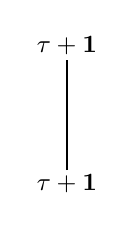
\begin{tikzpicture}[scale=0.7,baseline=(current bounding box.center)]
						\draw (0,-1) to (0,1);
						\node at (0,1.25) {\small $\tau+\mathbf{1}$};	
						\node at (0,-1.25) {\small $\tau+\mathbf{1}$};
					\end{tikzpicture}.
				\end{equation}
				The remaining coefficients can be determined by inserting the expression for $m_{\mathbf{1}+\tau}$ given above into \cref{eq:mcondpic}, which yields
					\begin{equation}
						\hspace{30pt}\begin{tikzpicture}[scale=0.8,baseline=(current bounding box.center)]
							\draw (0,0) to (90:1);
							\draw (0,0) to (230:1);
							\draw (0,0) to (310:1);	
							\draw[fill=LinkColor2!50!white] (0,0) circle(0.45cm);	
							\node (c) at (0,0) {\tiny $m_{\mathbf{1}+\tau}$};
							\node at (90:1.25) {\small $\mathbf{1}+\tau$};	
							\node at (230:1.25) {\small $\mathbf{1}+\tau$};
							\node at (310:1.25) {\small $\mathbf{1}+\tau$};	
							\begin{scope}[yshift=2.2cm, xshift=0.9cm]
							\draw (0,0) to (90:1);
							\draw (0,0) to (230:1);
							\draw (0,0) to (295:3.225);	
							\draw[fill=LinkColor2!50!white] (0,0) circle(0.45cm);	
							\node (c) at (0,0) {\tiny $m_{\mathbf{1}+\tau}$};
							\node at (90:1.25) {\small $\mathbf{1}+\tau$};	
							\node at (295:3.475) {\small $\mathbf{1}+\tau$};	
							\end{scope}
						\end{tikzpicture}\hspace{-10pt}={c_{\mathbf{1}\mathbf{1}}^\mathbf{1}}^2\fuselefttree{\mathbf{1}}{\mathbf{1}}{\mathbf{1}}{\mathbf{1}}{\mathbf{1}}+{c_{\tau\mathbf{1}}^\tau}^2\fuselefttree{\tau}{\mathbf{1}}{\tau}{\mathbf{1}}{\tau}+c_{\mathbf{1}\tau}^\tau c_{\tau\mathbf{1}}^\tau\fuselefttree{\mathbf{1}}{\tau}{\tau}{\mathbf{1}}{\tau}+\dots
					\end{equation}
				with $13$ terms in total and a similar expression for the right hand side of the equation. Consider those terms with diagrams in $\Hom(\tau\otimes\tau\otimes\tau,\tau)$ and apply $F$-moves to them:
				\begin{align}
					\hspace{10pt}&c_{\tau\tau}^\mathbf{1}c_{\mathbf{1}\tau}^\tau\fuselefttree{\tau}{\tau}{\mathbf{1}}{\tau}{\tau}+{c_{\tau\tau}^\tau}^2\fuselefttree{\tau}{\tau}{\tau}{\tau}{\tau}\\
					&\hspace{20pt}=\sum_xc_{\tau\tau}^\mathbf{1}c_{\mathbf{1}\tau}^\tau\left(F_\tau^{\tau\tau\tau}\right)_{x\mathbf{1}}\fuserighttree{\tau}{\tau}{x}{\tau}{\tau}+\sum_y{c_{\tau\tau}^\tau}^2\left(F_\tau^{\tau\tau\tau}\right)_{y\tau}\fuserighttree{\tau}{\tau}{y}{\tau}{\tau}.
				\end{align}
				Comparing this to the corresponding terms on the right hand side of the equation and setting $c_{\mathbf{1}\mathbf{1}}^\mathbf{1}=c_{\tau\mathbf{1}}^\tau=c_{\mathbf{1}\tau}^\tau=1$ yields the following system of equations:
				\begin{align}
					c_{\tau\tau}^\mathbf{1}&=c_{\tau\tau}^\mathbf{1}\left(F_\tau^{\tau\tau\tau}\right)_{\mathbf{1}\mathbf{1}}+{c_{\tau\tau}^\tau}^2\left(F_\tau^{\tau\tau\tau}\right)_{\mathbf{1}\tau}\\
					{c_{\tau\tau}^\tau}^2&=c_{\tau\tau}^\mathbf{1}\left(F_\tau^{\tau\tau\tau}\right)_{\tau\mathbf{1}}+{c_{\tau\tau}^\tau}^2\left(F_\tau^{\tau\tau\tau}\right)_{\tau\tau},
				\end{align}
				which has the following solution:
				\begin{align}
					c_{\tau\tau}^\mathbf{1}=\sqrt{2+\sqrt{5}}\ {c_{\tau\tau}^\tau}^2,
				\end{align}
				where $c_{\tau\tau}^\tau$ remains a free parameter since it is also not determined by checking the remaining equations. Hence, $\mathbf{1}+\tau$ is an algebra object in \textbf{Fib} with the multiplication morphism determined by the coefficients calculated above.
		\end{enumerate}	
\end{exmp}

Given an algebra object $A$ in a fusion category $\C$, one can build a \emph{module category} over $\C$ from it. For this purpose, we give an alternative definition of a module category in terms of the algebra object:
	\begin{defn}[Module over algebra object]
		\label{def:Amod}
		A left module over an algebra object $A$ in a category $\C$ (or, simply, a left $A$-module)\index{A-module@$A$-module} is a pair $(M,l)$ consisting of an object $M\in\C$ and a morphism $l:A\otimes M\to M$, depicted
			\begin{equation}
				\begin{tikzpicture}[baseline=(current bounding box.center)]
					\draw (0,0) to (90:1);
					\draw (0,0) to (230:1);
					\draw (0,0) to (310:1);	
					\draw[fill=LinkColor!50!white] (0,0) circle(0.3cm);	
					\node (c) at (0,0) {\small $l$};
					\node at (90:1.25) {\small $M$};	
					\node at (230:1.25) {\small $A$};
					\node at (310:1.25) {\small $M$};	
				\end{tikzpicture},
			\end{equation}
		such that it is compatible with the multiplication morphism $m$ of the algebra object, i.e., the following condition is fulfilled:
			\begin{align}
				l\circ(m\otimes\id_M)=l\circ(\id_A\otimes l)\hspace{10pt}\text{ as maps }A\otimes A\otimes M\to M \label{eq:MO1}.
			\end{align}
	\end{defn}

The constraint stated in \cref{eq:MO1} can be depicted as
\begin{equation}
	\begin{tikzpicture}[scale=0.85,baseline=(current bounding box.center)]
		\draw (0,0) to (90:1);
		\draw (0,0) to (230:1);
		\draw (0,0) to (310:1);	
		\draw[fill=LinkColor2!50!white] (0,0) circle(0.325cm);	
		\node (c) at (0,0) {\small $m$};
		\node at (90:1.25) {\small $A$};	
		\node at (230:1.25) {\small $A$};
		\node at (310:1.25) {\small $A$};	
		\begin{scope}[yshift=2.2cm, xshift=0.9cm]
		\draw (0,0) to (90:1);
		\draw (0,0) to (230:1);
		\draw (0,0) to (295:3.225);	
		\draw[fill=LinkColor!50!white] (0,0) circle(0.325cm);	
		\node (c) at (0,0) {\small $l$};
		\node at (90:1.25) {\small $M$};	
		\node at (295:3.475) {\small $M$};	
		\end{scope}
	\end{tikzpicture}=
	\begin{tikzpicture}[scale=0.85,baseline=(current bounding box.center)]
		\draw (0,0) to (90:1);
		\draw (0,0) to (230:1);
		\draw (0,0) to (310:1);	
		\draw[fill=LinkColor!50!white] (0,0) circle(0.325cm);	
		\node (c) at (0,0) {\small $l$};
		\node at (90:1.25) {\small $M$};	
		\node at (230:1.25) {\small $A$};
		\node at (310:1.25) {\small $M$};	
		\begin{scope}[yshift=2.2cm, xshift=-0.9cm]
		\draw (0,0) to (90:1);
		\draw (0,0) to (245:3.225);
		\draw (0,0) to (310:1);	
		\draw[fill=LinkColor!50!white] (0,0) circle(0.325cm);	
		\node (c) at (0,0) {\small $l$};
		\node at (90:1.25) {\small $M$};	
		\node at (245:3.475) {\small $A$};	
		\end{scope}
	\end{tikzpicture}.
\end{equation}

Analogously, one can define a right module over an algebra object $A\in\C$ via a morphism $r:M\otimes A\to M$ and the corresponding compatibility constraint.

	\begin{defn}[Module category over algebra object]
		The left $A$-modules in $\C$ form a category $\mathsf{Mod}_\C(A)$ whose objects consist of pairs $(M,l)$ given in \cref{def:Amod}\index{module category}. The morphisms in this category (also called $A$-left morphisms) are maps between module objects $(M_1,l_1)\to(M_2,l_2)$ that are compatible with the corresponding morphisms between $M_1,M_2$ in $\C$. More precisely, the following condition has to be fulfilled for $f\in\Hom_\C(M_1,M_2)$:
			\begin{equation}
			\label{eq:morphMod}
				f\circ l_1=l_2\circ(\id_A\otimes f)\hspace{10pt}\text{ as maps }A\otimes M_1\to M_2,
			\end{equation}
		depicted
			\begin{equation}
				\begin{tikzpicture}[scale=0.85,baseline=(current bounding box.center)]
					\draw (0,0) to (90:1);
					\draw (0,0) to (230:1);
					\draw (0,0) to (310:1);	
					\draw[fill=LinkColor!50!white] (0,0) circle(0.325cm);	
					\node (c) at (0,0) {\small $l_1$};
					\node at (90:1.25) {\small $M_1$};	
					\node at (230:1.25) {\small $A$};
					\node at (310:1.3) {\small $M_1$};
					\draw (0,1.5) -- (0,3);
					\draw[fill=LightGray] (0,2.25) circle(0.325cm);
					\node (d) at (0,2.25) {\small $f$};
					\node at (0,3.25) {$M_2$};
				\end{tikzpicture}=
				\begin{tikzpicture}[scale=0.85,baseline=(current bounding box.center)]
					\draw (0,0) to (90:1);
					\draw (0,0) to (230:1);
					\draw (0,0) to (310:1);	
					\draw[fill=LinkColor!50!white] (0,0) circle(0.325cm);	
					\node (c) at (0,0) {\small $l_2$};
					\node at (90:1.25) {\small $M_2$};	
					\node at (230:1.25) {\small $A$};
					\node at (310:1.3) {\small $M_2$};
					\draw (0.77,-2.75) -- (0.77,-1.25);
					\draw[fill=LightGray] (0.77,-2) circle(0.325cm);	
					\node (c) at (0.77,-2) {\small $f$};
					\draw (-0.77,-1.25) -- (-0.77,-2.75);
					\node at (-0.77,-3) {\small $A$};
					\node at (0.77,-3) {\small $M_1$};
				\end{tikzpicture}.
			\end{equation}
	\end{defn}

\begin{rem}
	\label{rem:Caction}
	Note that for any left $A$-module $(M,l)$ and any object $X\in\C$, we can define a functor $\circlearrowleft:\mathsf{Mod}_\C(A)\times \C\to\mathsf{Mod}_\C(A)$ via
		\begin{equation}
			(M,l)\circlearrowleft X=(M\otimes X,l\otimes \id_X).
		\end{equation}
	The object $M\otimes X$ has again the structure of a left $A$-module given by the composition
		\begin{equation}
			A\otimes(M\otimes A)=(A\otimes M)\otimes X\xrightarrow{l\otimes\id_X}M\otimes X.
		\end{equation}
	Hence, the category $\mathsf{Mod}_\C(A)$ is a right $\C$-module category in the sense of \cref{def:leftmod} with the right $\C$-action given by the functor $\circlearrowleft$. With the same argument, the category of right $A$-modules over $\C$ is a left $\C$-module category.
\end{rem}

In this way, we get a general construction of module categories from algebra objects in the category $\C$. An important question that immediately arises is whether every module category over $\C$ can be constructed in this way, and the answer is no. Consider the category $\mathsf{Vec}$ of all finite-dimensional vector spaces. The module category of \emph{all} vector spaces (which includes infinite dimensional ones) is not of the form $\mathsf{Mod}_{\C}(A)$. However, for $\C=\mathsf{Vec}$ any \emph{finite} module category is of the form $\mathsf{Mod}_{\mathsf{Vec}}(A)$. In general, it can be shown that all finite module categories over a finite monoidal category $\C$ are of the form $\mathsf{Mod}_{\mathsf{Vec}}(A)$ for a suitable algebra object $A$ (see \cite[Thm.\ 7.10.1]{Etingof2015} and \cite{Ostrik2003}).

With the definition of an $A$-module at hand we can rephrase the definition of bimodules in terms of algebra objects:
	\begin{defn}[Bimodule]
		Let $A,B$ be two algebra objects in a fusion category $\C$. An $A$--$B$ bimodule\index{bimodule} in $\C$ is a triple $(M,l_A,r_B)$ where $M\in\C$ and $l_A:A\otimes M\to M$, $r_B:M\otimes B\to M$ such that
			\begin{enumerate}
				\item The pair $(M,l_A)$ is a left $A$-module in $\C$.
				\item The pair $(M,r_B)$ is a right $B$-module in $\C$.
				\item The following condition is fulfilled:
						\begin{equation}
							r_B\circ(l_A\otimes\id_B)=l_A\circ(\id_A\otimes r_B),
						\end{equation}
					depicted
					\begin{equation}
					\begin{tikzpicture}[scale=0.85,baseline=(current bounding box.center)]
						\draw (0,0) to (90:1);
						\draw (0,0) to (230:1);
						\draw (0,0) to (310:1);	
						\draw[fill=LinkColor!50!white] (0,0) circle(0.325cm);	
						\node (c) at (0,0) {\small $l_A$};
						\node at (90:1.25) {\small $M$};	
						\node at (230:1.25) {\small $A$};
						\node at (310:1.25) {\small $M$};	
						\begin{scope}[yshift=2.2cm, xshift=0.9cm]
							\draw (0,0) to (90:1);
							\draw (0,0) to (230:1);
							\draw (0,0) to (295:3.225);	
							\draw[fill=LinkColor4!50!white] (0,0) circle(0.325cm);	
							\node (c) at (0,0) {\small $r_B$};
							\node at (90:1.25) {\small $M$};	
							\node at (295:3.475) {\small $B$};	
						\end{scope}
					\end{tikzpicture}=
					\begin{tikzpicture}[scale=0.85,baseline=(current bounding box.center)]
						\draw (0,0) to (90:1);
						\draw (0,0) to (230:1);
						\draw (0,0) to (310:1);	
						\draw[fill=LinkColor4!50!white] (0,0) circle(0.325cm);	
						\node (c) at (0,0) {\small $r_B$};
						\node at (90:1.25) {\small $M$};	
						\node at (230:1.25) {\small $M$};
						\node at (310:1.25) {\small $B$};	
						\begin{scope}[yshift=2.2cm, xshift=-0.9cm]
							\draw (0,0) to (90:1);
							\draw (0,0) to (245:3.225);
							\draw (0,0) to (310:1);	
							\draw[fill=LinkColor!50!white] (0,0) circle(0.325cm);	
							\node (c) at (0,0) {\small $l_A$};
							\node at (90:1.25) {\small $M$};	
							\node at (245:3.475) {\small $A$};	
						\end{scope}
					\end{tikzpicture}.
					\end{equation}
			\end{enumerate}
	\end{defn}
	
	\begin{rem}
		The $A$--$B$ bimodules in a category $\C$ form a category that we denote $\mathsf{Bimod}_\C(A,B)$. A morphism $f$ in this category is both an $A$-left morphism and a $B$-right morphism.
	\end{rem}

\begin{exmp}[Fibonacci category]
	\label{ex:FibMod}
	As shown in \cref{ex:AOFib}, the Fibonacci category \textbf{Fib}\index{Fibonacci category} has only two algebra objects: The trivial one $\mathbf{1}$ and $\mathbf{1}+\tau$ with multiplication morphism $m_{\mathbf{1}+\tau}$ given by
		\begin{equation}
			\begin{tikzpicture}[scale=0.9,baseline=(current bounding box.center)]
				\draw (0,0) to (90:1);
				\draw (0,0) to (230:1);
				\draw (0,0) to (310:1);	
				\draw[fill=LinkColor2!50!white] (0,0) circle(0.4cm);	
				\node (c) at (0,0) {\tiny $m_{\mathbf{1}+\tau}$};
				\node at (90:1.25) {\small $\mathbf{1}+\tau$};	
				\node at (230:1.25) {\small $\mathbf{1}+\tau$};
				\node at (310:1.25) {\small $\mathbf{1}+\tau$};	
			\end{tikzpicture}=
			\begin{tikzpicture}[scale=0.7,baseline=(current bounding box.center)]
				\draw (0,0) to (90:1);
				\draw (0,0) to (230:1);
				\draw (0,0) to (310:1);	
				\node at (90:1.25) {\small $\mathbf{1}$};	
				\node at (230:1.25) {\small $\mathbf{1}$};
				\node at (310:1.25) {\small $\mathbf{1}$};
			\end{tikzpicture}+
			\begin{tikzpicture}[scale=0.7,baseline=(current bounding box.center)]
				\draw (0,0) to (90:1);
				\draw (0,0) to (230:1);
				\draw (0,0) to (310:1);	
				\node at (90:1.25) {\small $\tau$};	
				\node at (230:1.25) {\small $\tau$};
				\node at (310:1.25) {\small $\mathbf{1}$};
			\end{tikzpicture}+
			\begin{tikzpicture}[scale=0.7,baseline=(current bounding box.center)]
				\draw (0,0) to (90:1);
				\draw (0,0) to (230:1);
				\draw (0,0) to (310:1);	
				\node at (90:1.25) {\small $\tau$};	
				\node at (230:1.25) {\small $\mathbf{1}$};
				\node at (310:1.25) {\small $\tau$};
			\end{tikzpicture}+\sqrt{2+\sqrt{5}}\ {c_{\tau\tau}^{\tau}}^2\hspace{-5pt}
			\begin{tikzpicture}[scale=0.7,baseline=(current bounding box.center)]
				\draw (0,0) to (90:1);
				\draw (0,0) to (230:1);
				\draw (0,0) to (310:1);	
				\node at (90:1.25) {\small $\mathbf{1}$};	
				\node at (230:1.25) {\small $\tau$};
				\node at (310:1.25) {\small $\tau$};
			\end{tikzpicture}+c_{\tau\tau}^{\tau}\hspace{-5pt}
			\begin{tikzpicture}[scale=0.7,baseline=(current bounding box.center)]
				\draw (0,0) to (90:1);
				\draw (0,0) to (230:1);
				\draw (0,0) to (310:1);	
				\node at (90:1.25) {\small $\tau$};	
				\node at (230:1.25) {\small $\tau$};
				\node at (310:1.25) {\small $\tau$};
			\end{tikzpicture}.
		\end{equation}
	We now show how to construct the category $\mathsf{Mod}_{\mathbf{Fib}}(\mathbf{1}+\tau)$ of left module objects over the algebra object $\mathbf{1}+\tau$. The technique we use here is described in \cite{grossman_quantum_2012}. We begin by determining all simple module objects with the following procedure: For this purpose, we calculate the fusion product of the algebra object $\mathbf{1}+\tau$ with all the simple objects in \textbf{Fib}, i.e., 
		\begin{equation}
			\label{eq:AfuseFib}
			A\otimes X_i
		\end{equation}
	for $X_i\in\{\mathbf{1},\tau\}$. We then build a matrix $T$ in the following way: Index each row and each column by a simple object $X_i\in\mathbf{Fib}$. A row of $T$ is given by the outcome of the fusion product \cref{eq:AfuseFib}, where the coefficients in the decomposition into simple objects are the entries in the row corresponding to the object $X_i$. For our example $A=\mathbf{1}+\tau$ we need to calculate
		\begin{align}
			\left(\mathbf{1}\otimes\tau\right)\otimes \mathbf{1}&=\mathbf{1}+\tau\\
			\left(\mathbf{1}\otimes\tau\right)\otimes \tau&=\tau+(\mathbf{1}+\tau)=\mathbf{1}+2\tau.
		\end{align}
	Hence, the matrix $T$ is of the form
		\begin{equation}
			T=\begin{blockarray}{ccc}
			& \mathbf{1} & \tau \\
			\begin{block}{c (cc)}
			\mathbf{1} & 1 & 1 \topstrut \\
			\tau & 1 & 2 \botstrut \\
			\end{block}
			\end{blockarray}\ .
		\end{equation} 
	It can be rewritten as
		\begin{equation}
			T=VV^\mathrm{T},
		\end{equation}
	where $V$ is the matrix that represents the action defined in \cref{rem:Caction}. Note that it is only possible to write $T$ in the form above if it is positive semidefinite, hence if this property is not fulfilled we can directly conclude that the corresponding object is not an algebra object. This matrix is the connection to the category of left modules: For a general fusion category $\C$ and a left module category $\mathsf{Mod}_\C(A)$ constructed from an algebra object $A$, the rows of $V$ are indexed by simple objects $X_i\in\C$ and the columns are indexed by simple objects $M_j\in\mathsf{Mod}_\C(A)$, hence $V$ is of the form
		\begin{equation}
		\label{eq:matrixV}
			V= \begin{blockarray}{ccccc}
			& M_1 & M_2 & M_3 & ...\\
			\begin{block}{c (cccc)}
			X_1 & ... & ... & ... & ... \topstrut\\
			X_2 & ... & ... & ... & ... \\
			X_3 & ... & ... & ... & ... \\
			... & ... & ... & ... & ... \botstrut\\
			\end{block}
			\end{blockarray}\ .
		\end{equation}
	This makes it possible to read off the decomposition of the simple module objects $M_j\in\mathsf{Mod}_\C(A)$ into simple objects $X_i\in\C$ from the columns of $V$. Therefore, we can determine all simple objects in $\mathsf{Mod}_\C(A)$ solely from the fusion outcomes of \cref{eq:AfuseFib}, i.e., from fusion rules in $\C$.
	
	For the algebra object $A=\mathbf{1}+\tau$ in \textbf{Fib} the matrix $V$ is of the form
		\begin{equation}
			V=\begin{pmatrix}
			1 & 0 \\
			1 & 1
			\end{pmatrix}.
		\end{equation}
	We can directly conclude that there are two simple module objects in the category $\mathrm{Mod}_{\mathbf{Fib}}(\mathbf{1}+\tau)$, which are
		\begin{align}
			M_1&=\mathbf{1}+\tau\\
			M_2&=\tau.
		\end{align}
	Note that the algebra object itself is always an object in the category of module objects, since it takes the place of the unit object here. The corresponding morphisms $l_{M_i}$ can be determined from the conditions given in \cref{def:leftmod} in a similar fashion to the procedure we used to determine the multiplication morphism $m_{\mathbf{1}+\tau}$ of the algebra object. The result for $M_1$ is simply the multiplication morphism $m_{\mathbf{1}+\tau}$, while $l_\tau$ is given by
		\begin{equation}
			\begin{tikzpicture}[scale=0.9,baseline=(current bounding box.center)]
				\draw (0,0) to (90:1);
				\draw (0,0) to (230:1);
				\draw (0,0) to (310:1);	
				\draw[fill=LinkColor!50!white] (0,0) circle(0.35cm);	
				\node (c) at (0,0) {\small $l_\tau$};
				\node at (90:1.25) {\small $\tau$};	
				\node at (230:1.25) {\small $\mathbf{1}+\tau$};
				\node at (310:1.25) {\small $\tau$};	
			\end{tikzpicture}=
			\begin{tikzpicture}[scale=0.7,baseline=(current bounding box.center)]
				\draw (0,0) to (90:1);
				\draw (0,0) to (230:1);
				\draw (0,0) to (310:1);	
				\node at (90:1.25) {\small $\tau$};	
				\node at (230:1.25) {\small $\mathbf{1}$};
				\node at (310:1.25) {\small $\tau$};
			\end{tikzpicture}-\frac{1+\sqrt{5}}{2}\ c_{\tau\tau}^\tau
			\begin{tikzpicture}[scale=0.7,baseline=(current bounding box.center)]
				\draw (0,0) to (90:1);
				\draw (0,0) to (230:1);
				\draw (0,0) to (310:1);	
				\node at (90:1.25) {\small $\tau$};	
				\node at (230:1.25) {\small $\tau$};
				\node at (310:1.25) {\small $\tau$};
			\end{tikzpicture}.
		\end{equation}
	Therefore, the category $\mathsf{Mod}_{\mathbf{Fib}}(\mathbf{1}+\tau)$ of left modules has two simple objects: $(\mathbf{1}+\tau,l_{\mathbf{1}+\tau})$ and $(\tau,l_\tau)$. Morphisms between these objects can be calculated by exploiting the condition \cref{eq:morphMod}. Analogously, the category of \emph{right} modules can be constructed from the algebra object $\mathbf{1}+\tau$ by building a matrix $T'$ using the fusion with the algebra object from the right side: $X_i\otimes A$. For the Fibonacci category this does not change the objects of the module category since the fusion rules are symmetric. The corresponding morphisms can be determined using the constraints from the definition of a right $A$-module category.
\end{exmp}

After explaining the construction of module categories via algebra objects, we can now understand the third point in \cref{prop:Morita}: If two categories $\C_1$ and $\C_2$ are Morita equivalent, then we can find an algebra object $A\in\C_1$ such that the category of $A$--$A$ bimodules constructed in the way described earlier is isomorphic to $\C_2$. 

As stated in the previous section, the two fusion categories arising from a finite depth subfactor are always Morita equivalent. However, it is possible that there exist other categories which are also Morita equivalent but not equivalent to these two. Hence, in general, there is a whole \emph{Morita equivalence class} of categories. In fact, the Morita equivalence class of the categories coming from the Haagerup subfactor contains a third category. This category, which we will encounter in \cref{ch:Haagerup}, is connected to the trivalent category $\Hd$ that was introduced in \cref{sec:H3triv} and hence has several nice properties. 


\section{From algebra objects to principal graphs}
\label{sec:AOtographs}

So far, we have discussed how to construct fusion categories from a given subfactor. It is also possible to go in the reverse direction: Beginning with a fusion category, one can construct all possible principal graphs by finding all algebra objects $A$ and the corresponding right $A$-module categories. The procedure goes as follows:
	\begin{enumerate}
		\item[1.] Find all algebra objects $A_i$ in a category $\C$.
		\item[2.] For each algebra object $A_i$, construct the category of right $A$-modules $\mathsf{Mod}_\C(A_i)$.
		\item[3.] For a fixed algebra object $A_i$, fix a simple module object $M_j$ in the module category $\mathsf{Mod}_\C(A_i)$.
		\item[4.] Calculate the action of each simple object $X_k\in\C$ on the fixed module object $M_j$, i.e., calculate $X_k\circlearrowright M_j$.
		\item[5.] Construct a graph in the following way: Write down all simple objects $X_k\in\C$ and all simple module objects $M_l\in\mathsf{Mod}_\C(A_i)$. For every time that a simple object $M_l$ appears in the decomposition of $X_k\circlearrowright M_j$ draw a line between $M_l$ and $X_k$.
	\end{enumerate}

Executing this procedure for all algebra objects and all simple module objects yields the collection of all principle graphs associated to the category $\C$.

\begin{exmp}[Fibonacci category]
	To illustrate the technique described above, consider once more the Fibonacci category \textbf{Fib}\index{Fibonacci category} and recall we have already found out about it: In \cref{ex:AOFib} we have calculated the algebra objects of \textbf{Fib}, which turned out to be $\mathbf{1}$ and $\mathbf{1}+\tau$ (step 1). In \cref{ex:FibMod} we have constructed the category of left $\mathbf{1}+\tau$-modules and pointed out that the category of right $\mathbf{1}+\tau$-modules has the same simple objects. Since for the construction of the principal graphs we are only interested in the objects and not the morphisms, we have completed step $2$ for the algebra object $\mathbf{1}+\tau$. The two simple module objects in $\textsf{Mod}_\mathbf{Fib}(\mathbf{1}+\tau)$ are $M_1=\mathbf{1}+\tau$ and $M_2=\tau$. We fix the module object $\mathbf{1}+\tau$ for this example (step 3). The action of the category \textbf{Fib} on this object (step 4) is then given by
		\begin{align}
			\mathbf{1}\circlearrowright(\mathbf{1}+\tau)&=\mathbf{1}+\tau=M_1\\
			\tau\circlearrowright(\mathbf{1}+\tau)&=\mathbf{1}+2\tau=M_1+M_2.
		\end{align}
	Following the construction explained in step $5$ yields the following principal graph: 
		\begin{equation}
		\label{eq:GraphFib}
			\begin{tikzpicture}[baseline=(current bounding box.center),scale=2.5]
				\draw (2,0) -- (3.5,0);
				\node at (2,0) {\color{LinkColor}\Large$\bullet$};
				\node at (3,0) {\color{LinkColor}\Large$\bullet$};
				\node at (2.5,0) {\color{LinkColor2}\Large$\bullet$};
				\node at (3.5,0) {\color{LinkColor2}\Large$\bullet$};
				\node at (2,-0.15) {\small $\mathbf{1}$};
				\node at (2.5,-0.15) {\small $M_1$};
				\node at (3,-0.15) {\small $\tau$};
				\node at (3.5,-0.15) {\small $M_2$};
			\end{tikzpicture}.
		\end{equation}
	This is the principal graph of the $A_4$ subfactor, which can be obtained from applying a construction by Popa \cite{Popa1990} to the module category described above. The $A_4$ subfactor has index $\dim(\mathbf{1}+\tau)=\frac{3+\sqrt{5}}{2}$ (see \cite{Jones2013} and references therein).
	
	Note that the adjacency matrix of the principal graph is also directly given by the matrix $V$ described in \cref{eq:matrixV}, since we fixed the module object in step (3) to be the algebra object itself. Hence, in case we are only interested in the principal graph that corresponds to the algebra object, but not in the other possible principle graphs (or the module category, as in \cref{ex:FibMod}), it suffices to construct the matrix $V$ and read off the graph from it directly. For the category \textbf{Fib} with the algebra object $\mathbf{1}+\tau$, we know from \cref{ex:FibMod} that
		\begin{equation}
			V=\begin{pmatrix}
				1 & 0 \\
				1 & 1
			\end{pmatrix},
		\end{equation}
	which is exactly the adjacency matrix of the graph given in \cref{eq:GraphFib}.
	
	The second possible principle graph (which cannot be read off from the matrix $V$ directly) is constructed by fixing the module object $\tau$ in step (3). The action of the simple objects in \textbf{Fib} is given by
		\begin{align}
			\mathbf{1}\circlearrowright\tau&=\tau=M_2\\
			\tau\circlearrowright\tau&=\mathbf{1}+\tau=M_1,
		\end{align}
	which yields the following graph:
		\begin{equation}
			\begin{tikzpicture}[baseline=(current bounding box.center),scale=2.5]
				\draw (2,0) -- (2.5,0);
				\draw (3,0) -- (3.5,0);
				\node at (2,0) {\color{LinkColor}\Large$\bullet$};
				\node at (3,0) {\color{LinkColor}\Large$\bullet$};
				\node at (2.5,0) {\color{LinkColor2}\Large$\bullet$};
				\node at (3.5,0) {\color{LinkColor2}\Large$\bullet$};
				\node at (2,-0.15) {\small $\mathbf{1}$};
				\node at (2.5,-0.15) {\small $M_2$};
				\node at (3,-0.15) {\small $\tau$};
				\node at (3.5,-0.15) {\small $M_1$};
			\end{tikzpicture}.
		\end{equation}
\end{exmp}

\section{The centre construction}
\label{sec:Drinfeld}

Given a monoidal category, one can construct the \emph{centre}\index{center} (also called \emph{Drinfeld centre}\index{Drinfeld centre}) of this category, which is the categorification of the centre of a ring. More detail on this construction can be found in \cite{muger_subfactors_2003,muger_subfactors_2003-1} and \cite{Etingof2015}. In the following, let $\C$ be a monoidal category with associator
	\begin{equation}
		\alpha_{X,Y,Z}:(X\otimes Y)\otimes Z\to X\otimes (Y\otimes Z).
	\end{equation}

	\begin{defn}
		The centre of a monoidal category $\C$ is the category $\mathcal{Z}(\C)$ defined as follows: The objects of $\mathcal{Z}(\C)$ are pairs $(Z,\gamma)$ where $Z\in\C$ and 
			\begin{equation}
				\gamma_X:X\otimes Z\to Z\otimes X,\hspace{10pt} X\in\C
			\end{equation}
		is a natural isomorphism called \emph{half-braiding}\index{half-braiding} such that the following diagram commutes for all $X,Y\in\C$:
			\begin{equation}
			\label{eq:halfb}
				\begin{tikzpicture}[scale=1.1,baseline=(current bounding box.center)]
					\node (1) at (0,0) {$X\otimes (Y\otimes Z)$};
					\node (2) at (2,1.5) {$X\otimes (Z\otimes Y)$};
					\node (3) at (6,1.5) {$(X\otimes Z)\otimes Y$};
					\node (4) at (8,0) {$(Z\otimes X)\otimes Y$};
					\node (5) at (2,-1.5) {$(X\otimes Y)\otimes Z$};
					\node (6) at (6,-1.5) {$Z\otimes(X\otimes Y)$};
					\draw[->] (1) to node[left] {\small $\id_X\otimes \gamma_Y$} (2);
					\draw[->] (2) to node[above] {\small $\alpha_{X,Z,Y}^{-1}$} (3);
					\draw[->] (3) to node[right] {\small $\ \gamma_X\otimes\id_Y$} (4);
					\draw[->] (1) to node[left] {\small $\alpha_{X,Y,Z}^{-1}$} (5);
					\draw[->] (5) to node[below] {\small $\gamma_{X\otimes Y}$} (6);
					\draw[->] (6) to node[right] {\small $\ \alpha_{Z,X,Y}^{-1}$} (4);
				\end{tikzpicture}
			\end{equation}
		A morphism from $(Z,\gamma)$ to $(Z',\gamma')$ is a morphism $f\in\Hom_\C(Z,Z')$ such that for each $X\in\C$ the following condition is fulfilled:
			\begin{equation}
				\label{eq:centermorph}
				(f\otimes \id_X)\circ\gamma_X=\gamma_X'\circ(\id_X\otimes f),
			\end{equation}
		which can be depicted
		\begin{equation}
			\begin{tikzpicture}[scale=0.9,baseline=(current bounding box.center)]
				\node (X) at (0,0) {$X$};
				\node (Z) at (1,0) {$Z$};
				\node (Z2) at (0,2) {$Z$};
				\node (X2) at (1,2) {$X$};
				\node (Z3) at (0,4) {$Z'$};
				\node (X3) at (1,4) {$X$};
				\draw (X) -- (Z2);
				\draw (Z) -- (X2);
				\draw (Z2) -- (Z3);
				\draw (X2) -- (X3);
				\draw[fill=LightGray, draw=black, rounded corners] (-0.25,0.75) rectangle (1.25,1.25);
				\node at (0.5,1) {\small $\gamma_X$};
				\draw[fill=LightGray, draw=black] (0,3) circle (0.3cm);
				\node at (0,3) {\small $f$};
			\end{tikzpicture}\ =\ 
			\begin{tikzpicture}[scale=0.9,baseline=(current bounding box.center)]
				\node (X) at (0,0) {$X$};
				\node (Z) at (1,0) {$Z$};
				\node (Z2) at (0,2) {$X$};
				\node (X2) at (1,2) {$Z'$};
				\node (Z3) at (0,4) {$Z'$};
				\node (X3) at (1,4) {$X$};
				\draw (X) -- (Z2);
				\draw (Z) -- (X2);
				\draw (Z2) -- (Z3);
				\draw (X2) -- (X3);
				\draw[fill=LightGray, draw=black, rounded corners] (-0.25,2.75) rectangle (1.25,3.25);
				\node at (0.5,3) {\small $\gamma'_X$};
				\draw[fill=LightGray, draw=black] (1,1) circle (0.3cm);
				\node at (1,1) {\small $f$};
			\end{tikzpicture}\ .
		\end{equation}
	\end{defn}
	
	The centre of a monoidal category is again a monoidal category. The tensor product in this category is given as follows: For two objects $(Z,\gamma)$, $(Z',\gamma')$ in $\mathcal{Z}(\C)$ it is defined as
		\begin{equation}
			(Z,\gamma)\otimes (Z',\gamma')=(Z\otimes Z',\tilde{\gamma})
		\end{equation}
	with
		\begin{equation}
			\tilde{\gamma}_X:X\otimes(Z\otimes Z')\to(Z\otimes Z')\otimes X,\hspace{10pt}X\in\C
		\end{equation}
	given by the following commuting diagram:
		\begin{equation}
			\begin{tikzpicture}[scale=1.1,baseline=(current bounding box.center)]
				\node (1) at (0,0) {$X\otimes(Z\otimes Z')$};
				\node (2) at (4,0) {$(X\otimes Z)\otimes Z'$};
				\node (3) at (8,0) {$(Z\otimes X)\otimes Z'$};
				\node (4) at (8,-2) {$Z\otimes(X\otimes Z')$};
				\node (5) at (4,-2) {$Z\otimes(Z'\otimes X)$};
				\node (6) at (0,-2) {$(Z\otimes Z')\otimes X$};
				\draw[->,>=stealth] (1) to node[above] {\small $\alpha_{X,Z,Z'}^{-1}$} (2);
				\draw[->,>=stealth] (2) to node[above] {\small $\gamma_X\otimes\id_{Z'}$} (3);
				\draw[->,>=stealth] (3) to node[right] {\small $\alpha_{Z,X,Z'}$} (4);
				\draw[->,>=stealth] (4) to node[above] {\small $\id_Z\otimes\gamma_X'$} (5);
				\draw[->,>=stealth] (5) to node[above] {\small $\alpha_{Z,Z',X}^{-1}$} (6);
				\draw[->,>=stealth] (1) to node[left] {\small $\tilde{\gamma}_X$} (6);
			\end{tikzpicture}
		\end{equation}
	The unit object in $\mathcal{Z}(\C)$ is $(\mathbf{1},r^{-1}l)$, where $r$ and $l$ are the right and left unit constraints of the underlying monoidal category $\C$.
	
	\begin{rem}
		If the category $\C$ is strict, condition \cref{eq:halfb} simplifies to 
			\begin{equation}
				\gamma_{X\otimes Y}=(\gamma_X\otimes\id_Y)\circ(\id_X\otimes \gamma_Y)
			\end{equation}
		and the half-braiding $\tilde{\gamma}_X$ of the tensor product is given by
			\begin{equation}
				\tilde{\gamma}_X=(\id_Z\otimes\gamma_X')\circ(\gamma_X\otimes\id_{Z'}).
			\end{equation}
	\end{rem}

The main reason why the centre construction is of interest to the work described in this thesis is because of the following theorem which was proved in \cite{muger_subfactors_2003-1}:
	\begin{thm}
		The centre $\mathcal{Z}(\C)$ of a spherical fusion category $\C$ is a modular tensor category.
	\end{thm}

The above theorem provides a way to construct a modular tensor category from a spherical fusion category, which is especially interesting with regard to the fusion categories associated to the Haagerup subfactor since these categories are not modular themselves. It is therefore a powerful tool in our search for a conformal field theory that corresponds to the Haagerup subfactor: From the modular tensor category, we can construct an anyon chain and investigate whether is has any critical points, which themselves are possibly described by a conformal field theory. This is described in more detail in \cref{sec:anyons}.